
\section{Integrating \calculus with Object Oriented Languages}
\label{sct:scala-translation}
\usetikzlibrary{arrows, decorations.markings}
% for double arrows a la chef
% adapt line thickness and line width, if needed
\tikzstyle{vecArrow} = [thick, decoration={markings,mark=at position
   1 with {\arrow[semithick]{open triangle 60}}},
   double distance=1.4pt, shorten >= 5.5pt,
   preaction = {decorate},
   postaction = {draw,line width=1.4pt, white,shorten >= 4.5pt}]
\tikzstyle{innerWhite} = [semithick, white,line width=1.4pt, shorten >= 4.5pt]

\begin{figure}
\center
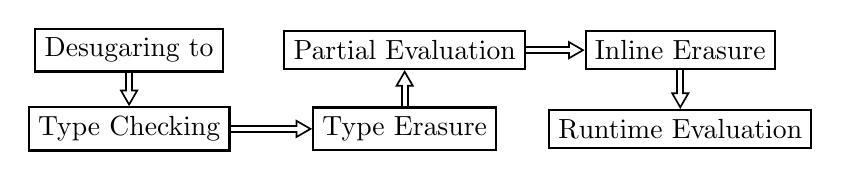
\begin{tikzpicture}[thick]
  \node[draw,rectangle] (a) {Desugaring to \calculus};
  \node[draw,rectangle,below of=a, node distance = 1.0cm] (b) {Type Checking \calculus};
  \node[draw,rectangle,right of=b, node distance = 3.5cm] (c) {Type Erasure};
  \node[draw,rectangle,right of=a, node distance = 3.5cm] (d) {Partial Evaluation};
  \node[draw,rectangle,right of=d, node distance = 3.5cm] (e) {Inline Erasure};
  \node[draw,rectangle,right of=c, node distance = 3.5cm] (f) {Runtime Evaluation};

  % 1st pass: draw arrows
  \draw[vecArrow] (a) to (b);
  \draw[vecArrow] (b) to (c);
  \draw[vecArrow] (c) to (d);
  \draw[vecArrow] (d) to (e);
  \draw[vecArrow] (e) to (f);

  % Note: If you have no branches, the 2nd pass is not needed
\end{tikzpicture}
\caption{Compilation pipeline.}
\label{fig:phases}
\end{figure}

% Description of the chapter

The \calculus calculus \sct{sct:calculus} captures the essence of user-controlled
 predictable partial-evaluation. In practice, though, it is fairly low level and
 it is not obvious how to define \emph{classes} and methods from in modern multi-paradigm
 programming languages. Furthermore, \calculus requires an inconveniently
 large number of \code{inline} calls in method invocations.
 In this section we a scheme for translating classes into \calculus (\sct{sct:desugaring}),
 show how to provide compile time views of classes and and \emph{methods}\sct{sct:promotion},
 and formalize convenient implicit conversions for the calculus \sct{sct:conversions}.

% Restricted Language
Furthermore, rules of \calculus do not support effect-full computations and each
 \code{inline} term is trivially converted to a dynamic term after erasure.
 In case of languages that do support mutable state and side-effects this needs to
 be treated specially. For simplicity, we omit side-effects from our discussion and
 assume that all partially evaluated code is side-effect free and that each
 \code{inline} term can be converted to dynamic code.

% Method signatures
\subsection{Desugaring Object Oriented Constructs to \calculus}
\label{sct:desugaring}

\begin{figure}
\begin{alignat*}{2}
   & [\![ \klet\ x: T_x = t_x\ \kin \ t ]\!] = ((x: T_x) \ra t)(t_x)\\
   & [\![ \klet\ type\ T_1 = T_2\ \kin\ t ]\!] =  ([T_1 <: T_2] \ra t)[T_2] \\
   & [\![ \klet\ class\ C[A](x: T_x) \{ def\ f[B](y: T_y) = t_f \}\ \kin\ t ]\!]  =  \\
   & \quad   \klet\ type\  C = [A] \ra \inline \{ fields: \{ x: T_x \}, methods: \inline \{ f: [B] \ra T_y \ra T_f \}\ \} \kin  \\
   & \quad \quad \klet\ C: [A] \ra \inline((t_x: T_x) \ra C[A])  =  [A] \ra \inline((t_x: T_x) \ra\\
   & \quad \quad \quad  \inline \{ fields = \{x = t_x\}, methods = \inline \{f = [B] \ra (y: T_y) \ra t_f \}\}) \ \kin\ t
\end{alignat*}
\caption{Desugaring of classes into \calculus.}
\label{fig:desugaring-classes}
\end{figure}


\subsection{Compile-Time View of the Terms}
\label{sct:compile-views}
\begin{figure}
\begin{multicols}{2}[]

  \infrule[\textsc{CT-TVar}]
    {\Pi \ts T \in \Pi}
    {\Pi \ts \cd{iT}{iT}}

  \infrule[\textsc{CT-T-Var}]
    {\Pi \ts T \not\in \Pi}
    {\Pi \ts \cd{iT}{\inline{T}}}

\end{multicols}
\vspace{4pt}

  \infrule[\textsc{CT-Rec}]
    {\seq{\Pi \ts \cd{t}{t'}}}
    {\Pi \ts \cd{\i\{ \seq{x = t} \}}{\inline{\{ \seq{x = t'} \}}}}

  \infrule[\textsc{CT-T-Rec}]
    {\seq{\Pi \ts \cd{\i{T}}{\j{T}}}}
    {\Pi \ts \cd{\{\seq{x : \i{T}}\}}{\inline{\{ \seq{x : \j{T}}}\}}}

  \infrule[\textsc{CT-T-Arrow}]
    {\Pi \ts \cd{\i{T}}{\j{T}} \ \ \ \  \Pi \ts \cd{\k{S}}{\l{S}} }
    {\Pi \ts \cd{\i{T} \Rightarrow \k{S}}{\j{T} \Rightarrow \l{S}}}

  \infrule[\textsc{CT-T-Univ}]
    {\Pi \ts \cd{\j{T}}{\k{T}}}
    {\Pi \ts \cd{[X <: \i{S}] \ra \j{T}}{[X <: \i{S}] \ra \k{T}}}

  \infrule[\textsc{CT-Func}]
    {\Pi \ts \cd{t}{t'} \ \ \ \ \Pi \ts \cd{iT}{jT}}
    {\Pi \ts \cd{\i(x: iT) \ra t}{\inline{(x: jT) \ra t'}}}

  \infrule[\textsc{CT-TAbs}]
    {\Pi,\ X \ts \cd{t}{t'}}
    {\Pi \ts \cd{\i([X <: \j{T_1}] \ra t)}{\inline{([X <: \j{T_1}] \ra t'})}}

  \infrule[\textsc{CT-TApp}]
    {\Pi \ts \cd{t}{t'} \ \ \ \ \Pi \ts \cd{\i{T}}{\j{T}}}
    {\Pi \ts \cd{t[\i{T}]}{t'[\j{T}]}}

\caption{Translation of a type abstractions, function, and record values into a compile-time view. The translation
 is used for promoting types into their compile time versions.}
\label{fig:partial-evaluation}
\end{figure}

\subsection{Implicit Conversions}
\label{sct:conversions}

% Requires desugaring
According to \calculus rules if method signatures contain compile-time views of a type
 the corresponding arguments in method application would always have to be promoted to \code{inline}.
 In practice this is not convenient as it requires an inconveniently large number
 of annotations. Partial evaluation is an optimization, and as such, it should not
 affect user code - users should not be aware of the internal operation of the library.

To address this issue we introduce implicit conversions from all language literals, and
 straight class constructor calls of non-inline type into their compile-time views.
 For example, for a factorial function \begin{lstparagraph}
def fact(n: Int @ct) = if (n == 0) 1 else fact(n - 1)
 \end{lstparagraph} we will not require annotations on literals \code{0}, and \code{1}. Furthermore,
 the function can be invoked without promoting the literal \code{5} into it's compile-time view:\begin{lstparagraph}
fact(5)
  $\hookrightarrow$ 120
 \end{lstparagraph}
